\documentclass{article}

\title{Counting Bloom filter}
\author{Gerard Martin Teixidor}

\usepackage{graphicx}

\usepackage[parfill]{parskip}

\begin{document}
\maketitle

\section*{Description}
A Bloom filter~\cite{bloom} is a probabilistic data structure which allows to test whether an element is a member of a set. While Bloom filters does not allow to remove elements, Counting Bloom filter~\cite{counting} is an extension of the original data structure which allows the delete operation. Notice that Counting bloom filters represent a multiset instead of a set. Both Bloom filters are considered probabilistic since false positive matches are possible, but false negative matches are not.

A Bloom filter is a bit array of $m$ bits initially all set to $0$. When an element is inserted, $k$ hash functions map the element to $k$ different positions, setting the bit of those positions to $1$. To check if an element is in the set, as the insert operation, the element hashed against $k$ hash functions to retrieve the position. If all positions are set to $1$, the elements belongs to the set. Notice that those bits could be set to $1$ because the insertion of other elements, being a false positive.

Given the probability of false positives $\epsilon$ and the number of inserted elements $n$, the optimal number of bits is $m = \frac{-n\ln\epsilon}{\ln^2 2}$. Meanwhile, the optimal number of hash functions is $k=-\log_2\epsilon$.

\begin{figure}[h]
\centering
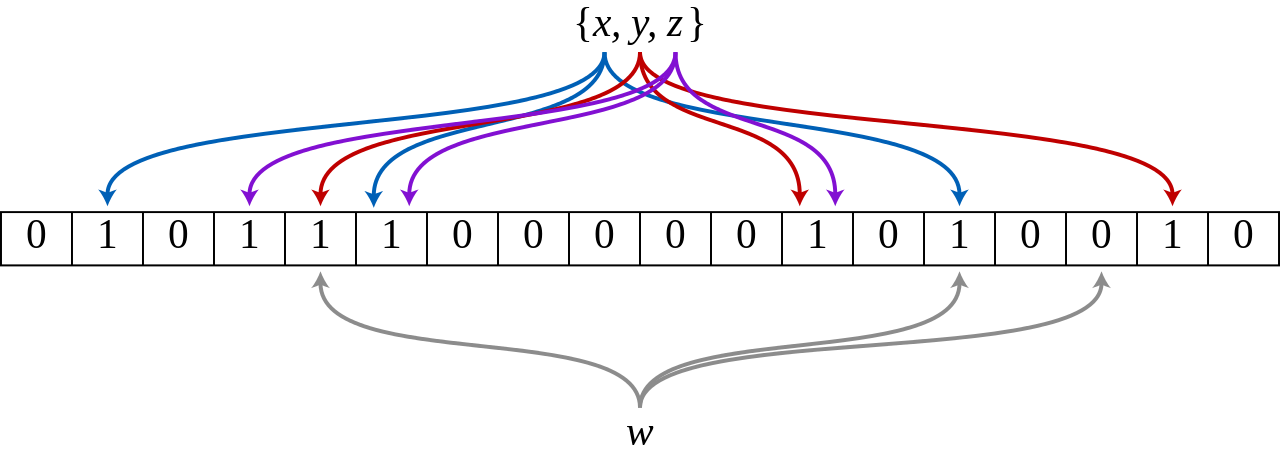
\includegraphics[width=0.8\linewidth]{bloom_filter.png}
\label{fig:bloom_filter}
\caption{Example of a Bloom filter representing the set $\{x, y ,z\}$. Using $3$ hash functions, each element is mapped to $3$ positions. The element $w$ is not in the set since one of the mapped position contains a $0$.}
\end{figure}

To implement a Counting Bloom filter, the only change required is to substitute the bit array for an integer array. When we insert an element, instead of setting the bit to $1$, we increment the bits, while removing an element we decrement the bits. To check if an element belongs to the set, all bits must be greater than~$0$.

\section*{Implementation}
The implemented Counting Bloom filter only accepts strings as elements of the multiset. The example provided shows how it can be used to test if a word belongs to the input text.

\subsection*{Operations}
List of the implemented operations with a brief description and their time complexity:

\paragraph*{\textit{insert}} Insert a string.
\begin{description}
\item[] Time complexity: $O(1)$
\end{description}

\paragraph*{\textit{erase}} Erase an string. Can return a false positive.
\begin{description}
\item[] Time complexity: $O(1)$
\end{description}

\paragraph*{\textit{contains}} Test whether the collection contains a string. Can return a false positive.
\begin{description}
\item[] Time complexity: $O(1)$
\end{description}

\bibliographystyle{unsrt}
\bibliography{report.bib}

\end{document}